\begin{figure}[t]
    \begin{subfigure}{0.19\textwidth}
        \centering
        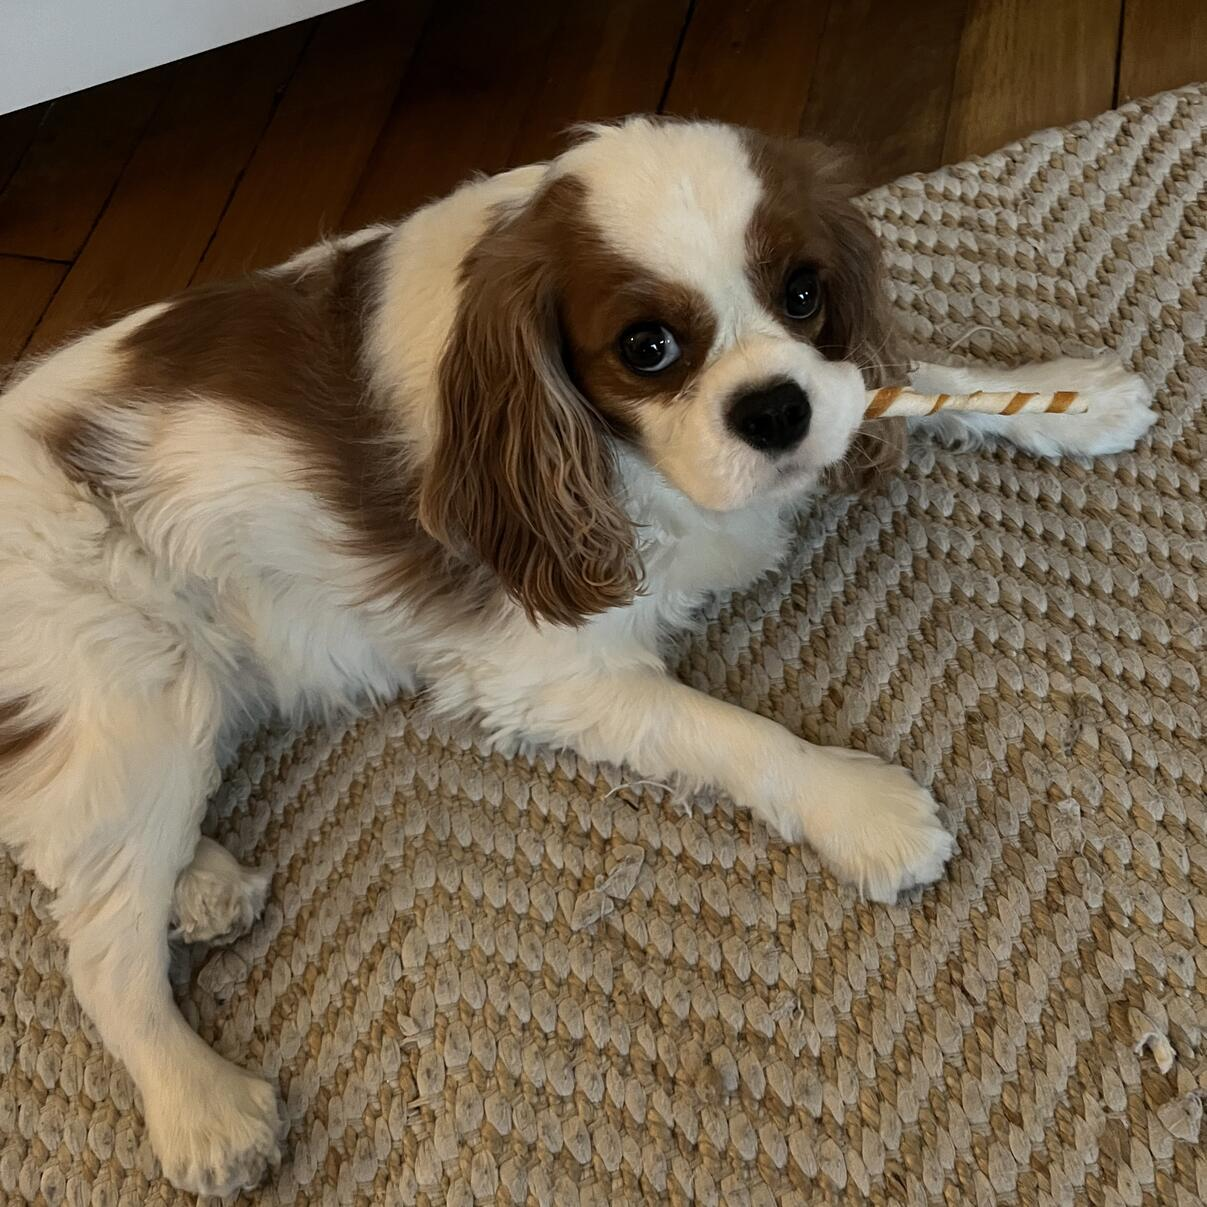
\includegraphics[width=\linewidth]{figures/analysis/highres/dog_pca_vit7b/dog.lr.jpeg}
        \caption*{Input}
    \end{subfigure}\hfill
    \begin{subfigure}{0.19\textwidth}
        \centering
        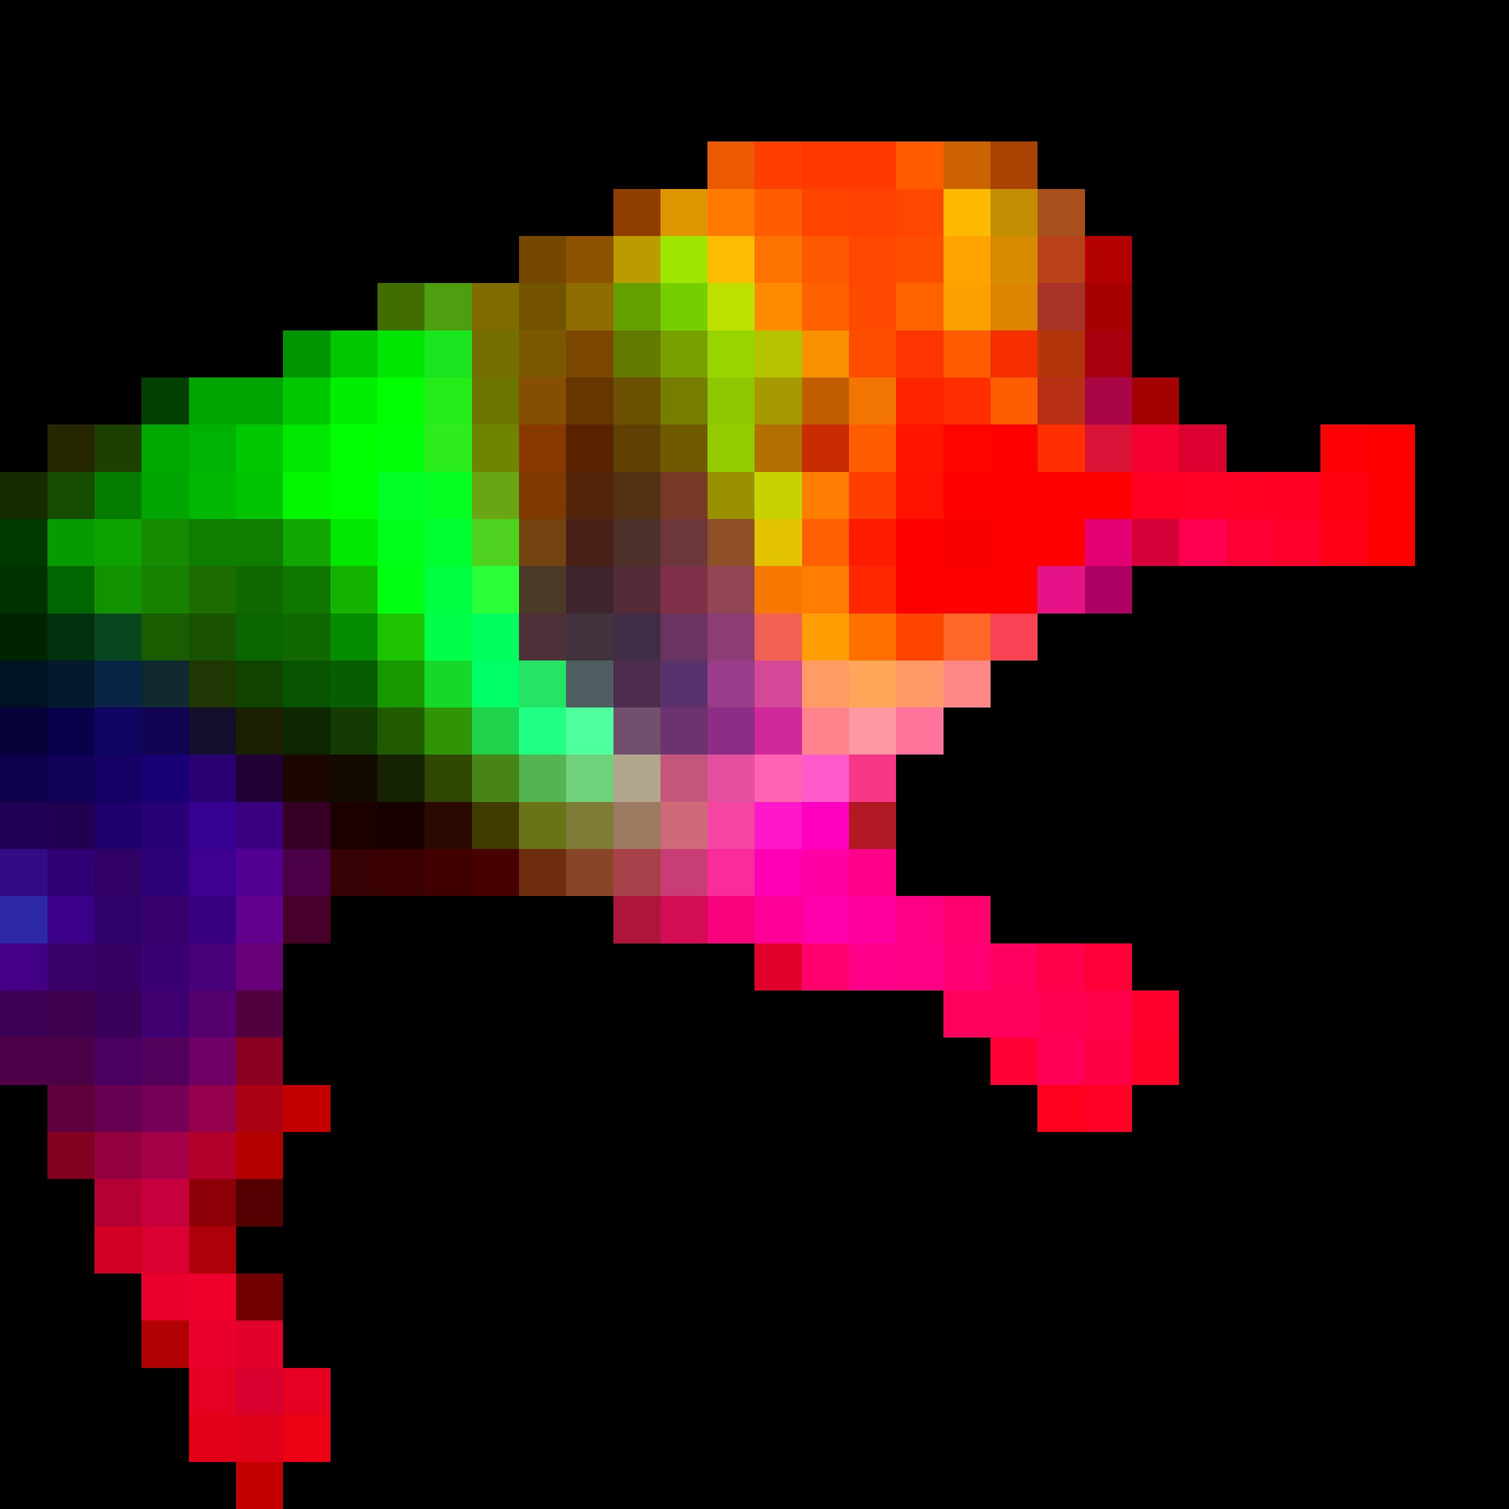
\includegraphics[width=\linewidth]{figures/analysis/highres/dog_pca_vit7b/dog_512.lr.png}
        \caption*{$512 \times 512$}
    \end{subfigure}\hfill
    \begin{subfigure}{0.19\textwidth}
        \centering
        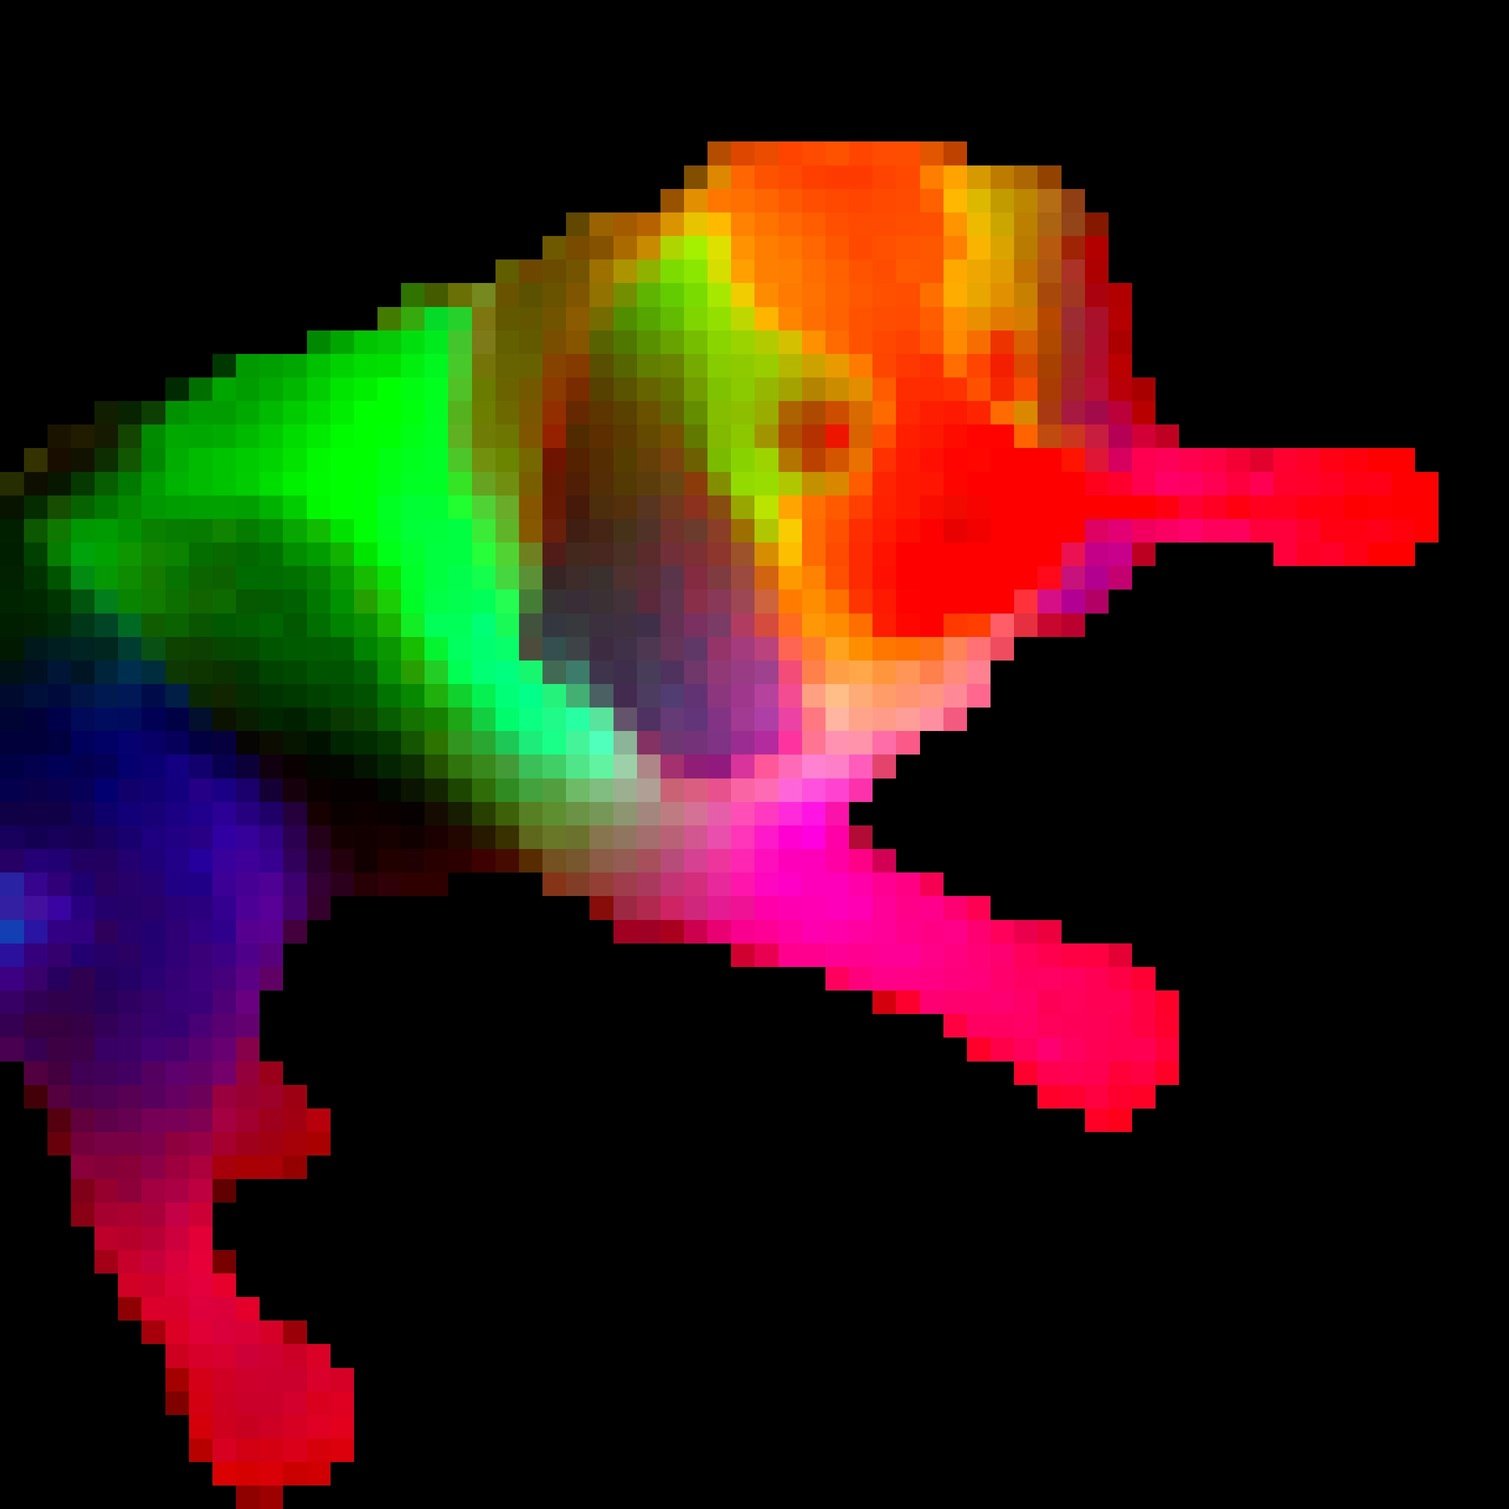
\includegraphics[width=\linewidth]{figures/analysis/highres/dog_pca_vit7b/dog_1024.lr.jpeg}
        \caption*{$1024 \times 1024$}
    \end{subfigure}\hfill
    \begin{subfigure}{0.19\textwidth}
        \centering
        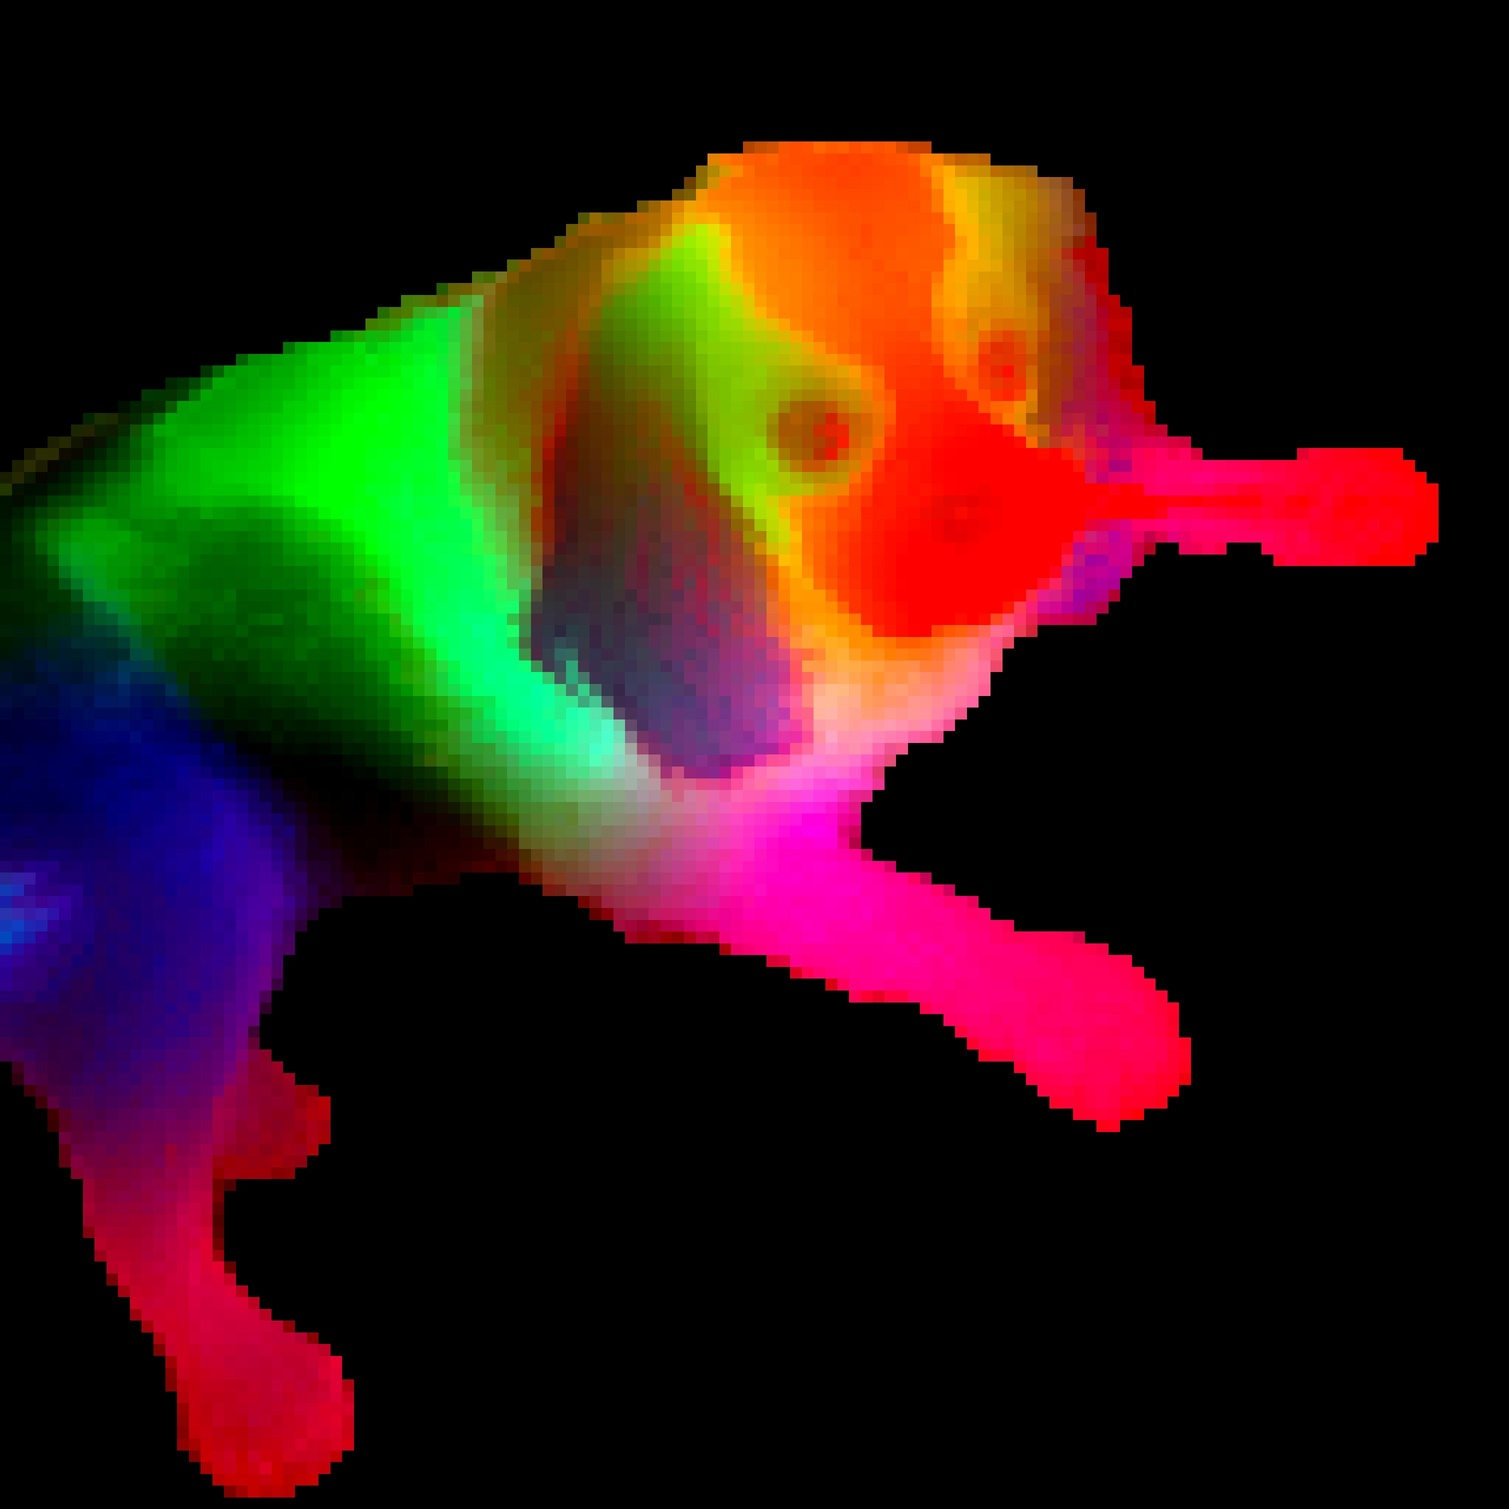
\includegraphics[width=\linewidth]{figures/analysis/highres/dog_pca_vit7b/dog_2048.lr.jpeg}
        \caption*{$2048 \times 2048$}
    \end{subfigure}\hfill
    \begin{subfigure}{0.19\textwidth}
        \centering
        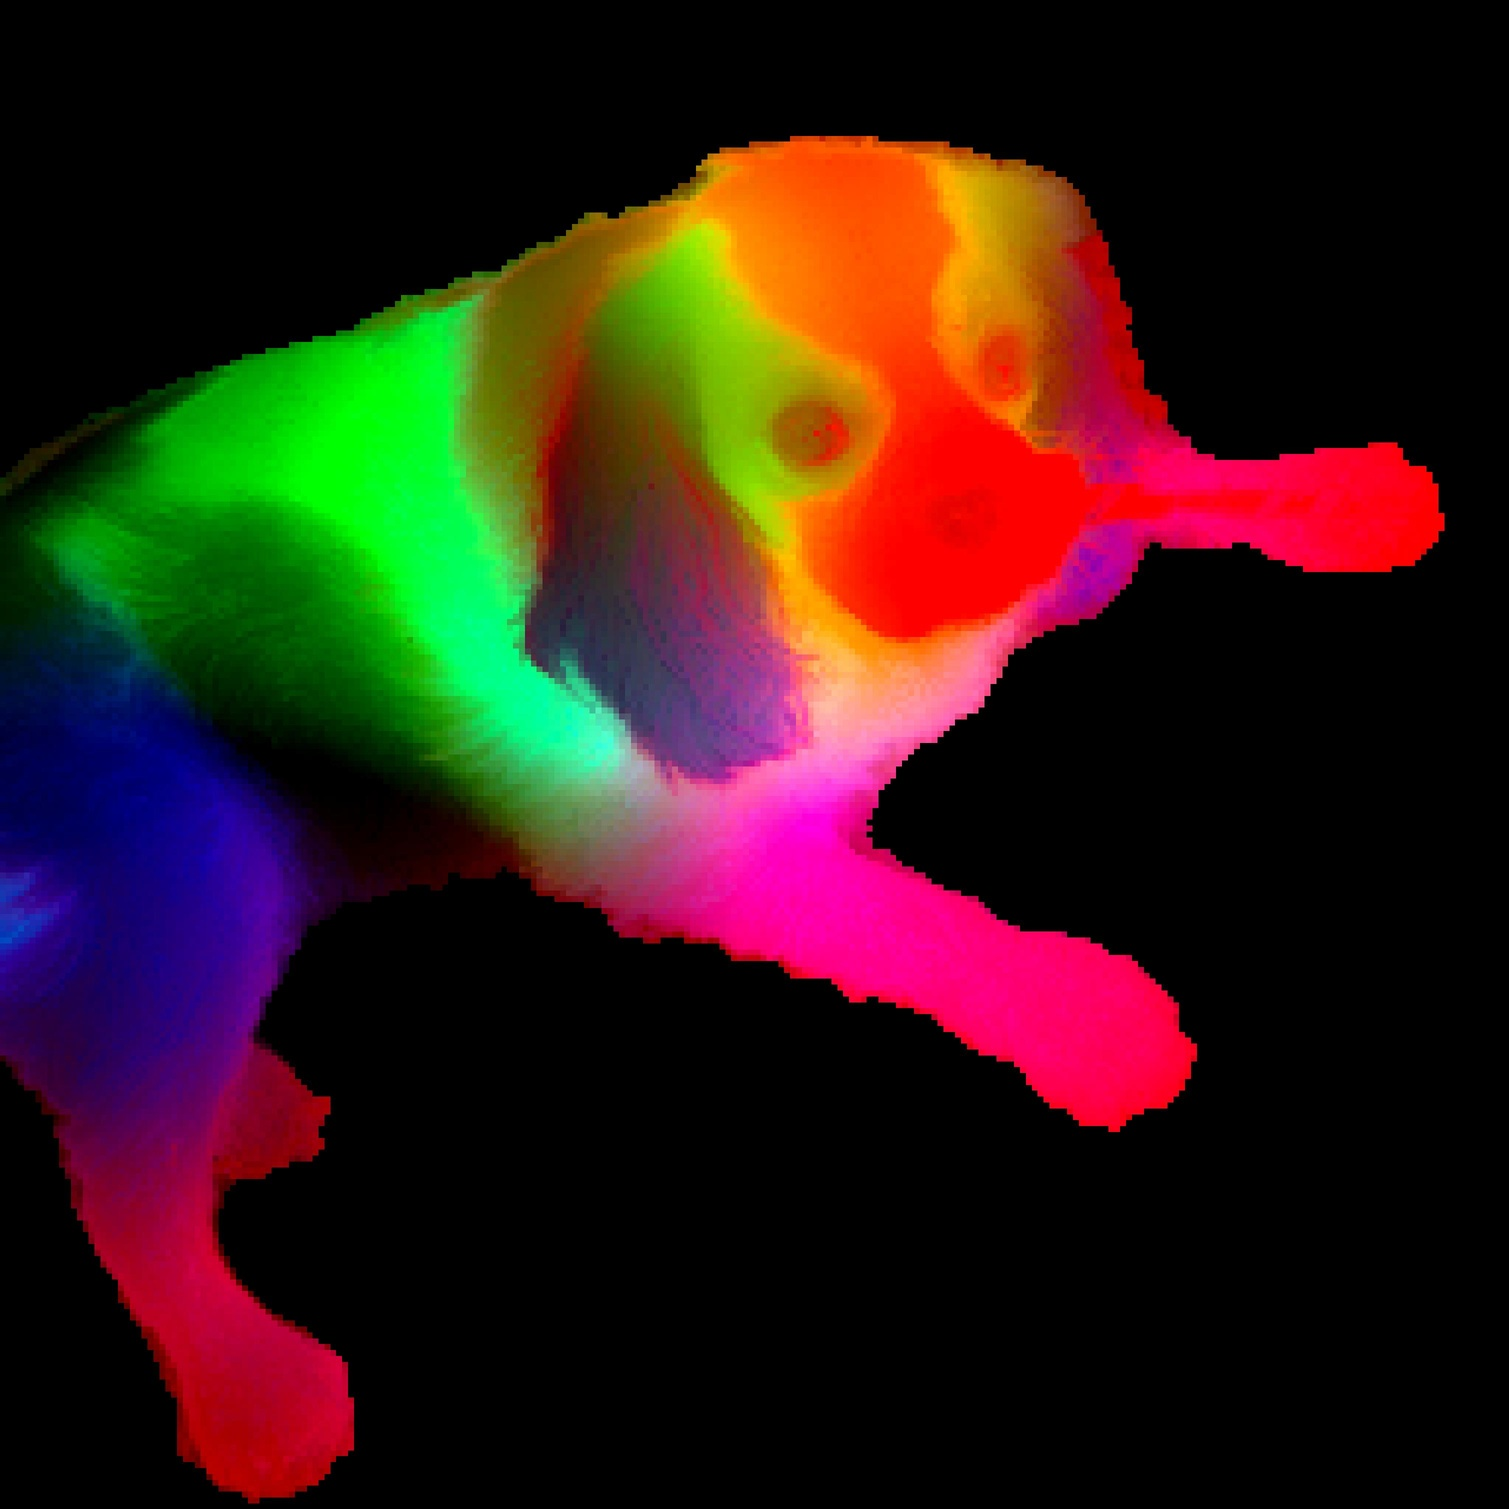
\includegraphics[width=\linewidth]{figures/analysis/highres/dog_pca_vit7b/dog_4096.lr.jpeg}
        \caption*{$4096 \times 4096$}
    \end{subfigure}%
    \caption{
        DINOv3 at very high resolution. 
        We visualize dense features of DINOv3 by mapping the first three components of a PCA computed over the feature space to RGB.
        To focus the PCA on the subject, we mask the feature maps via background subtraction.
        With increasing resolution, DINOv3 produces crisp features that stay semantically meaningful.
        We visualize more PCAs in \cref{sec:results-qualitative}.
    }
    \label{fig:visualization-extreme-resolutions}
\end{figure}

